\documentclass[a4paper,12pt]{article}
\usepackage[utf8]{inputenc}
\usepackage[italian]{babel}
\usepackage{amsmath}
\usepackage{amsthm}
\usepackage{color}
\usepackage{listings}
\usepackage{graphicx}
\usepackage{float}

\graphicspath{{./Confronti}}
\lstset{
    language=Python,
    keywordstyle=\color{blue},
    breaklines=true
    }

\title{Progetto Intelligenza Artificiale}
\author{Gianluca Parpanesi}
\begin{document}
    \maketitle
    \begin{abstract}
        \textit{"Confronto tra ARIMA e Tensorflow LSTM su titoli azionari"}
    \end{abstract}
    \newpage
    \section*{Introduzione}Il progetto ha lo scopo di mettere a confronto due 
    tecniche di regressione per apprendere e predire un'andamento di una 
    specifica azione (scelta dall'utente).
    Le tecniche utilizzate sono le seguenti:
    \begin{itemize}
        \item \textbf{ARIMA}: modello matematico-statistico basato su serie 
        temporali di dati. La parte Autoregressiva (AR) indica che la variabile
        di interesse viene regredita su valori precedenti (numero di intervalli
        di tempo). L'integrazione (I) indica che i valori dei dati sono stati 
        sostituiti con la differenza tra i loro valori e i valori dei 
        precedenti (volte in cui i dati sono stati sottratti ai valori passati)
        . Infine la media mobile (MA) indica che l'errore di regressione è in 
        realtà una combinazione lineare di termini di errore i cui valori si 
        sono verificati contemporaneamente e in tempi differenti in passato.
        ARIMA combina le caratteristiche autoregressive con quelle delle medie 
        mobili. Un processo autoregressivo AR(1), ad esempio, è quello in cui il 
        valore corrente è basato sul valore immediatamente precedente, 
        mentre un processo AR(2) è quello in cui il valore corrente è basato 
        sui due valori precedenti. Una media mobile è un calcolo utilizzato per
        analizzare i punti dati creando una serie di medie di diversi 
        sottoinsiemi dell'intero set di dati per attenuare l'influenza dei 
        valori anomali. Come risultato di questa combinazione di tecniche, i 
        modelli ARIMA possono tenere conto di tendenze, cicli, stagionalità e 
        altri tipi di dati non statici quando si effettuano previsioni.
        \footnote[1]{fonte: Wikipedia/ARIMA, Investopedia/ARIMA}
        \item LSTM: rete neurale ricorrente (\textit{RNN - Recurrent Neural 
        Network}) applicabile a processi di classificazione, serie temporali e 
        predizione. Una unità LSTM (\textit{LSTM - Long Short Term Memory}) è 
        componsto una singola cella con un input, un output e un \textit{forget
        gate}. La cella ricorda i valori di una serie temporale arbitraria e 
        l'input e il forget regolano il flusso di informazioni entranti nella
        singola cella. Il forget decide quale informazione deve essere scartata
        confrontando lo stato precedente con il valore attuale ed assegnandoli
        un valore [0, 1]. L'input decide quale parte di informazioni mantenere
        mentre l'output (come detto dal nome stesso), lascia passare un valore
        (basato sull'input e sul forget).\footnote[2]{fonte: Wikipedia/LSTM}

    \end{itemize}

    \section*{Struttura del codice}Il codice, scritto in Python, permette 
    di selezionare un'azione (o un ETF / fondo) che si desidera analizzare.
    All'interno del codice è possibile regolare degli
    \textit{iperpametri} in modo da regolare in base alle proprie esigenze
    la quantità dei dati da scaricare, regolare ARIMA e regolare Tensorflow
    (compresi i singoli parametri della RNN).

    \section{Avvio del programma}La parte iniziale ci permette di scaricare
    un titolo di mercato a nostra scelta mediante la libreria 
    \lstinline|yfinance|\footnote[3]{pypi.org/project/yfinance/}, la quale 
    scarica i dati direttamente dalle API pubbliche di Yahoo Finance i dati
    del titolo da noi richiesto. Il titolo viene ricercato tramite il 
    Ticker (abbreviazione utilizzata per identificare un titolo, 
    \textit{es: Apple Inc. = AAPL, Microsoft = MSFT}), scaricando i dati
    in un lasso di tempo identificato da un iperparametro 
    \lstinline|PERIOD|.
    \begin{lstlisting}[frame=single]
    ...            
    yf.Ticker(input("Quale titolo vuoi scaricare?\n"))
    ...
    history = data.history(PERIOD)
    \end{lstlisting}
    

    \section{Struttura del codice}Una volta scaricati i dati del titolo 
    richiesto verranno passati a due metodi, uno che avvierà l'analisi tramite 
    ARIMA mentre l'altro tramite Tensorflow (LSTM). Per entrambi è possibile 
    impostare un iperparametro \lstinline|SIZE| il quale identifica come 
    verranno suddivisi i dati. Precisamente \lstinline|SIZE| è un valore
    in percentuale che indentifica la porzione di dati riservata alla fase
    di \textit{training} del modello (ARIMA/Tensorflow LSTM), il restante
    verrà utilizzato come porzione di \textit{test}.

        \subsection{ARIMA}Il file \lstinline|arima.py| dispone di tre 
        iperparametri per il settaggio delle tre componenti ARIMA ovvero,
        come spiegato in precedenza, AR - Autoregressive, I - Integrated,
        MA - Moving Average, strettamente maggiori di 0. Il modello è 
        costruito tramite la libreria stastmodel, importando il modello 
        ARIMA\footnote[5]{statsmodels.tsa.arima.model.ARIMA}.

\begin{lstlisting}[frame=single]

    def ARIMA_Predictions(data: pd.DataFrame):

        values = data.values
        size = int(len(values)*SIZE)
        train = values[0:size]
        test = values[size:len(values)]
        history = [x for x in train]
        predictions = list()
    
        for x in range(len(test)):
    
            model_fit = create_model(history)
            output = model_fit.forecast()
            pred = output[0]
            predictions.append(pred)
            obs = test[x]
            history.append(obs)
    

        sqm = sqrt(mean_squared_error(test, predictions))

        return predictions, sqm
    
\end{lstlisting}

        \subsection{Tensorflow LSTM}La rete neurale LSTM viene costruita 
        tramite la libreria Tensorflow\footnote[6]{www.tensorflow.org} 
        basata su Keras, ovvero una libreria open source di apprendimento 
        automatico. La rete è multilivello, strutturata nel seguente modo:
        \begin{itemize}
            \item LSTM
            \item DROPOUT
            \item LSTM
            \item DROPOUT
            \item LSTM
            \item DROPOUT
            \item DENSE
        \end{itemize}
        La rete è stata sviluppata multilivello per rendere più solido 
        l'addestramento, soprattutto con pochi dati, a discapito di una
        computazione maggiore. Anche il file \lstinline|tens.py| dispone
        di alcuni iperparametri per regolare tutti i settaggi della rete.
        Gli iperparametri utilizzati per la rete neurale sono i seguenti:
        \begin{itemize}
            \item EPOCHS: il numero di passi di addestramento effettuati 
            dalla rete.
            \item PREDICTION DAY: indica la granularità sulla quale la rete
            effettua l'addestramento, un valore più alto comporta una 
            precisione minore.
            \item UNITS: indica la dimensione interna di una cella LSTM.
            \item DROPOUT: valore compreso tra 0 e 1 che permette di 
            decidere la percentuale di nodi interni scartati in una rete 
            neurale in fase di addestramento.
            \item DENSE: indica la dimensionalità dell'output.
        \end{itemize}
        I dati vengono normalizzati e suddivisi in dati di train e di test
        basandosi sulla proporzione scelta dall'utente, dettata
        dall'iperparametro \lstinline|SIZE|. Una volta suddivisi verranno
        create varie coppie (input, output) in modo da apprendere il 
        modello e testarlo successivamente con i dati di test. La 
        dimensione del blocco di dati assegnato all'input è determinato, 
        come detto in precedenza, da \lstinline|PREDICITON DAY|.
\begin{lstlisting}[frame = single]

    for a in range(PREDICTION_DAY, len(train)):

        #es: da 0 - 30, 30, coppia (x, y) dato x -> risultato y
        #es: da 1 - 31, 31

        train_x.append(train[a-PREDICTION_DAY:a, 0])
        train_y.append(train[a, 0])
    
\end{lstlisting}
        Successivamente viene creato il modello utilizzato nella creazione
        della rete neurale multilivello. Il modello è di tipo 
        \lstinline|Sequential()|, ovvero un modello adatto per una pila di 
        strati piana dove ogni strato ha esattamente un tensore di ingresso
        ed uno di uscita.
        Creato quindi il modello base, andremo ad aggiungere i vari strati
        della rete nell'ordine specificato in precedenza:
\begin{lstlisting}[frame = single]

    model = Sequential()
    model.add(LSTM(units = UNITS, return_sequences = True, input_shape=(train_x.shape[1], 1)))
    model.add(Dropout(DROPOUT))
    model.add(LSTM(units = UNITS, return_sequences=True))
    model.add(Dropout(DROPOUT))
    model.add(LSTM(units = UNITS))
    model.add(Dropout(DROPOUT))
    model.add(Dense(units = DENSE))
    model.summary()
    model.compile(optimizer = "adam", loss="mean_squared_error")
    
\end{lstlisting}
        Come funzione di loss utilizziamo la stessa utilizzata per il 
        modello ARIMA. Successivamente passeremo i dati suddivisi in
        precedenza, avendo quindi la rete pronta ad essere addestrata e 
        valutata.

    \section{Inizio analisi} Confronteremo ora l'analisi effettuata da ARIMA e 
    Tensorflow LSTM sull'azione Microsoft in un periodo pari a 5 anni
    (\lstinline|PERIOD = "5Y"|). Una volta scaricati i dati verrà avviata 
    automaticamente l'analisi prima di ARIMA e successivamente di Tensorflow.
    Ai fini di un confronto più accurato proveremo vari settaggi di vari 
    iperparametri per entrambi. Partiremo con dei valori di default per poi 
    incrementarli ad ogni confronto effettuato. Entrambi utilizzeranno un 
    rapporto 0.70 di size.

        \subsection{Primo confronto}
            \subsubsection{Analisi ARIMA} I valori utilizzati di default sono i
            segueti:
            \begin{itemize}
                \item Autoregressive: 5
                \item Integrated: 1
                \item Moving Average: 0 
            \end{itemize}
            \subsubsection{Analisi Tensorflow LSTM} I valori utilizzati di 
            default sono i seguenti:
            \begin{itemize}
                \item EPOCHS: 5
                \item PREDICTION DAY: 30
                \item UNITS: 64
                \item DROPOUT: 0.5
                \item DENSE: 1 (rimarrà tale per tutti gli altri addestramenti)
            \end{itemize}
            \subsubsection{Confronto}
                \begin{figure}[H]
                    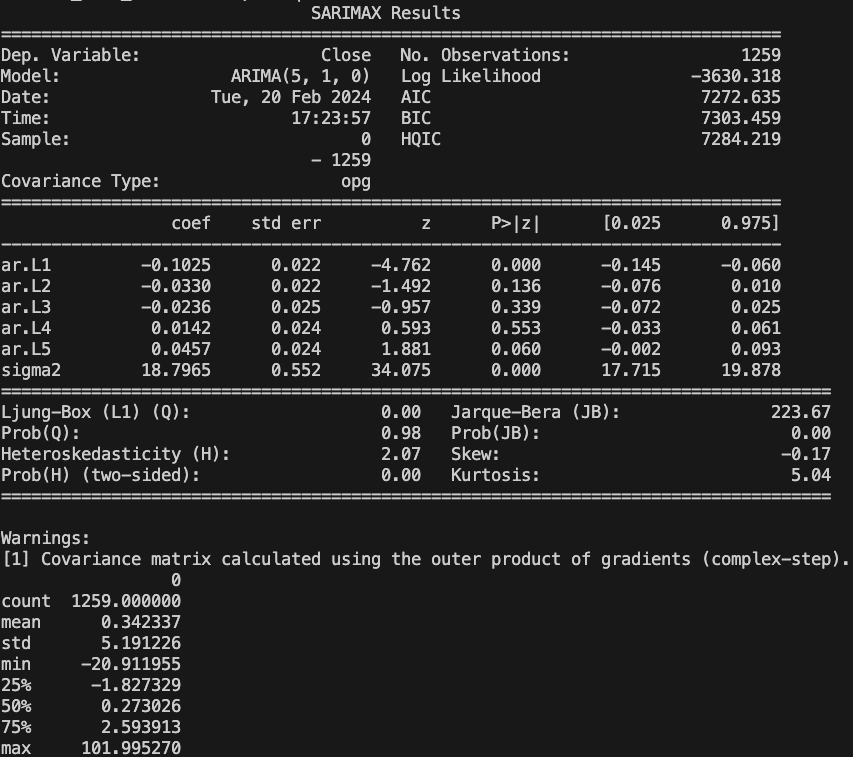
\includegraphics[width=\textwidth]{ARIMA1.png}
                    \caption{Risultati analisi preliminare della libreria 
                    ARIMA}
                \end{figure}
                \begin{figure}[H]
                    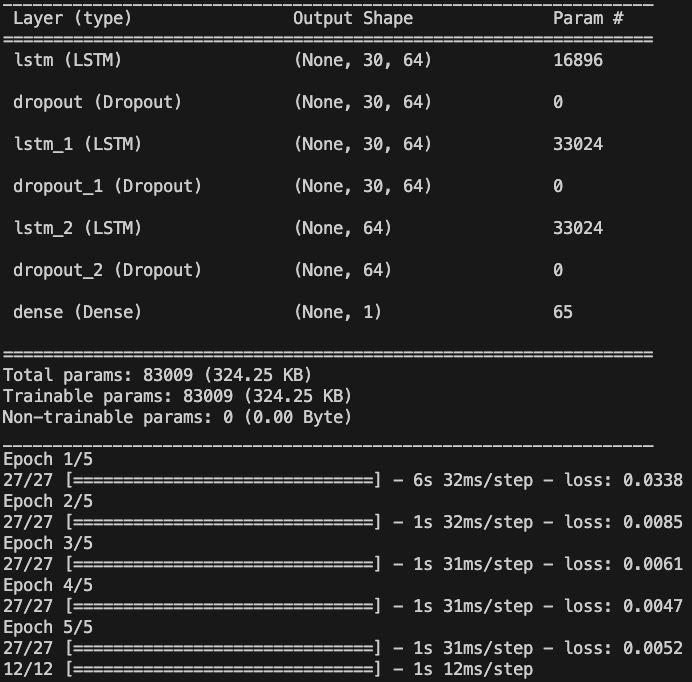
\includegraphics[width=\textwidth]{LSTM1.png}
                    \caption{Struttura Rete Neurale e passi di apprendimento}
                \end{figure}
                \begin{figure}[H]
                    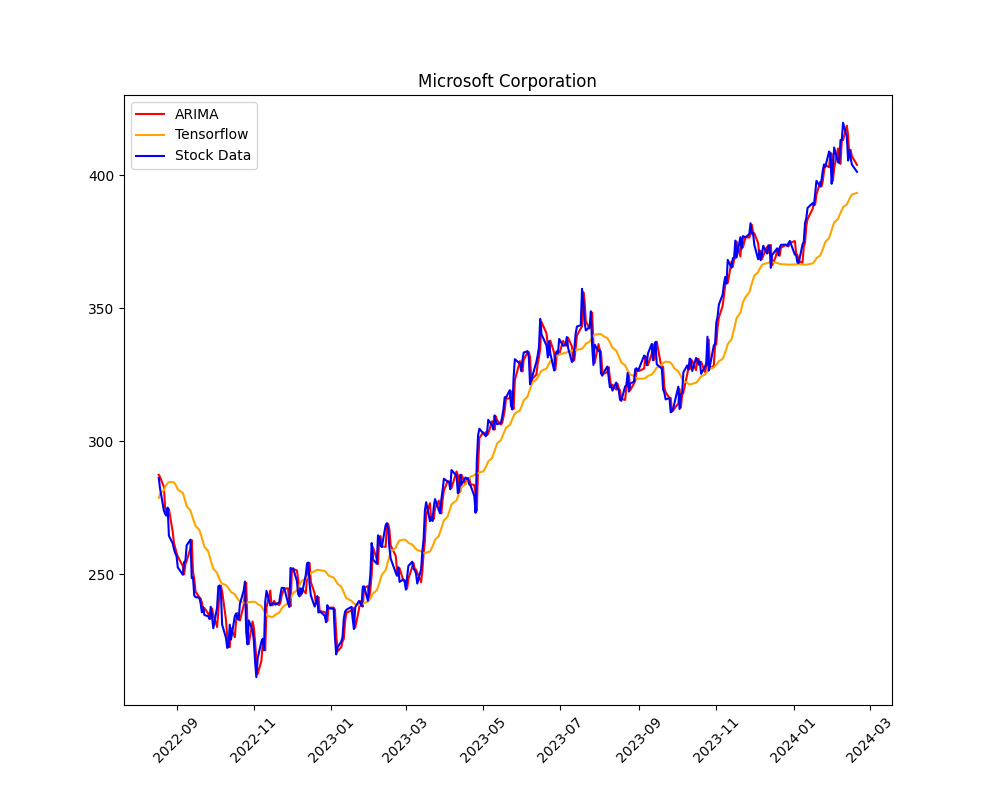
\includegraphics[width=\textwidth]{GRAFICO1.png}
                    \caption{Confronto tra apprendimento ARIMA e LSTM}
                \end{figure}
            I risultati ottenuti, confrontati tramite scarto quadratico medio
            sono i seguenti:
            \begin{figure}[H]
                \centering
                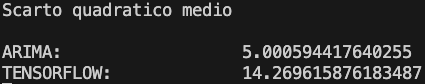
\includegraphics[width=0.5\textwidth]{SQM1.png}
                \caption{Confronti tra gli scarti quadratici medi}
            \end{figure}

        \newpage

        \subsection{Secondo confronto}
            \subsubsection{Analisi ARIMA} I valori utilizzati di default sono i
            segueti:
            \begin{itemize}
                \item Autoregressive: 10
                \item Integrated: 2
                \item Moving Average: 0 
            \end{itemize}
            \subsubsection{Analisi Tensorflow LSTM} I valori utilizzati di 
            default sono i seguenti:
            \begin{itemize}
                \item EPOCHS: 10
                \item PREDICTION DAY: 15
                \item UNITS: 128
                \item DROPOUT: 0.3
            \end{itemize}
            \subsubsection{Confronto}
            \begin{figure}[H]
                \centering
                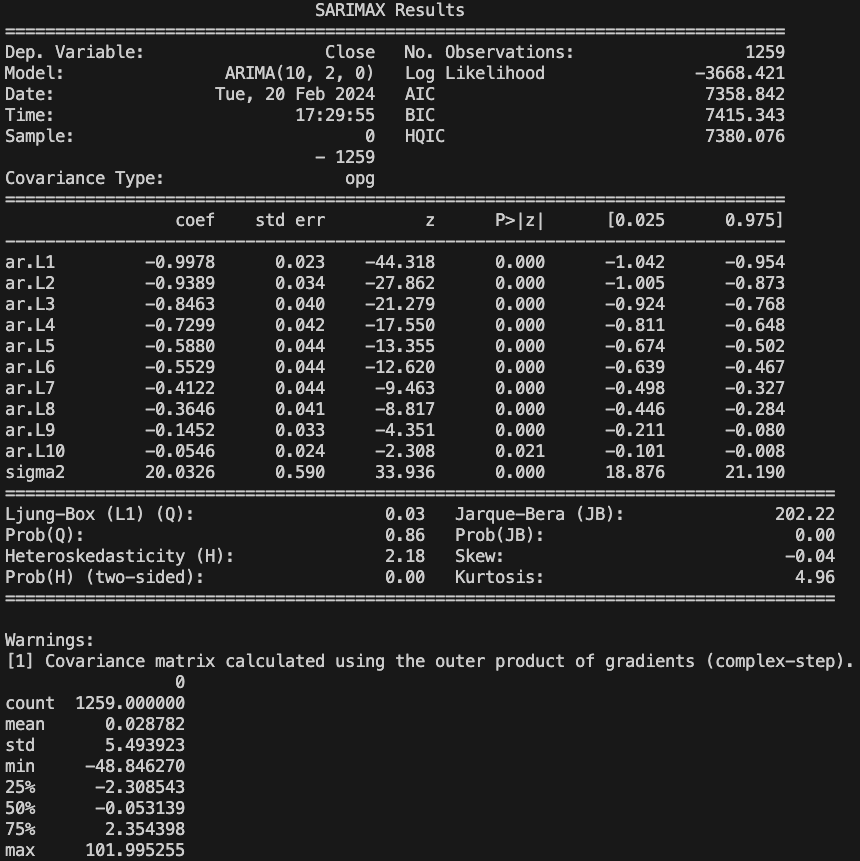
\includegraphics[width=0.9\textwidth]{ARIMA2.png}
                \caption{Risultati analisi preliminare della libreria 
                ARIMA}
            \end{figure}
            \begin{figure}[H]
                \centering
                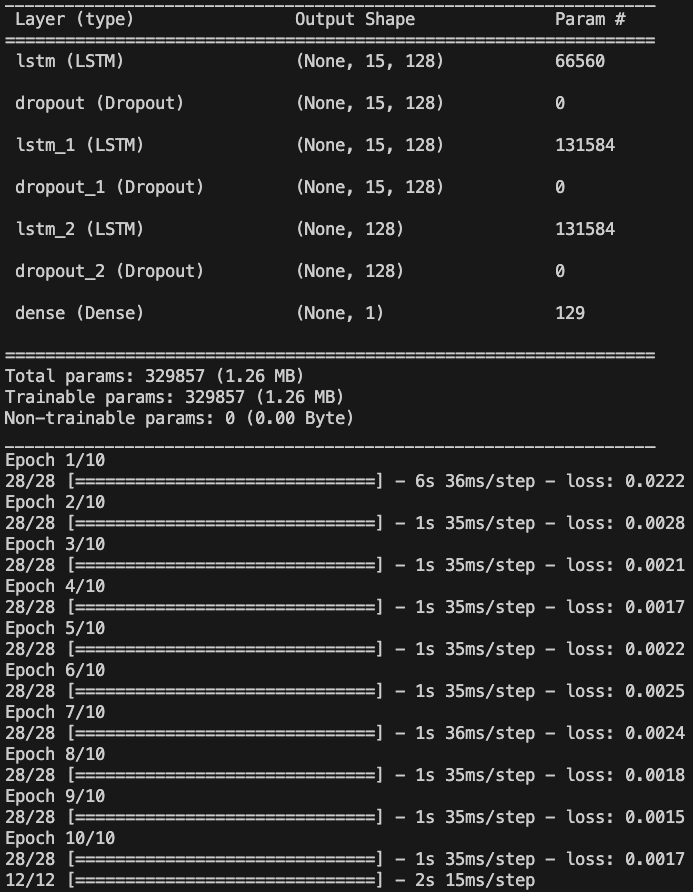
\includegraphics[width=0.9\textwidth]{LSTM2.png}
                \caption{Struttura Rete Neurale e passi di apprendimento}
            \end{figure}
            \begin{figure}[H]
                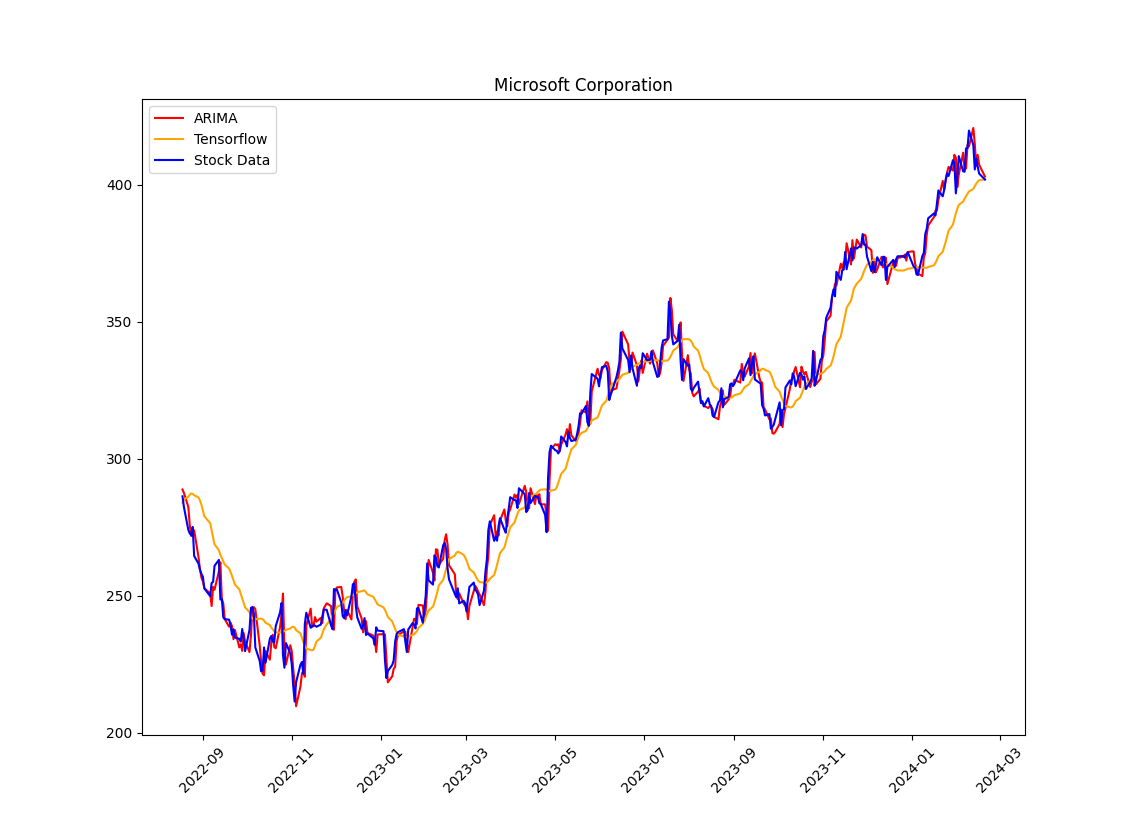
\includegraphics[width=\textwidth]{GRAFICO2.png}
                \caption{Confronto tra apprendimento ARIMA e LSTM}
            \end{figure}
            I risultati ottenuti, confrontati tramite scarto quadratico medio
            sono i seguenti:
            \begin{figure}[H]
                \centering
                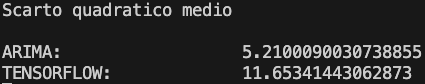
\includegraphics[width=0.5\textwidth]{SQM2.png}
                \caption{Confronti tra gli scarti quadratici medi}
            \end{figure}

        \newpage

        \subsection{Terzo confronto}
            \subsubsection{Analisi ARIMA} I valori utilizzati di default sono i
            segueti:
            \begin{itemize}
                \item Autoregressive: 20
                \item Integrated: 4
                \item Moving Average: 0 
            \end{itemize}
            \subsubsection{Analisi Tensorflow LSTM} I valori utilizzati di 
            default sono i seguenti:
            \begin{itemize}
                \item EPOCHS: 20
                \item PREDICTION DAY: 7
                \item UNITS: 256
                \item DROPOUT: 0.2
            \end{itemize}
            \subsubsection{Confronto}
            \begin{figure}[H]
                \centering
                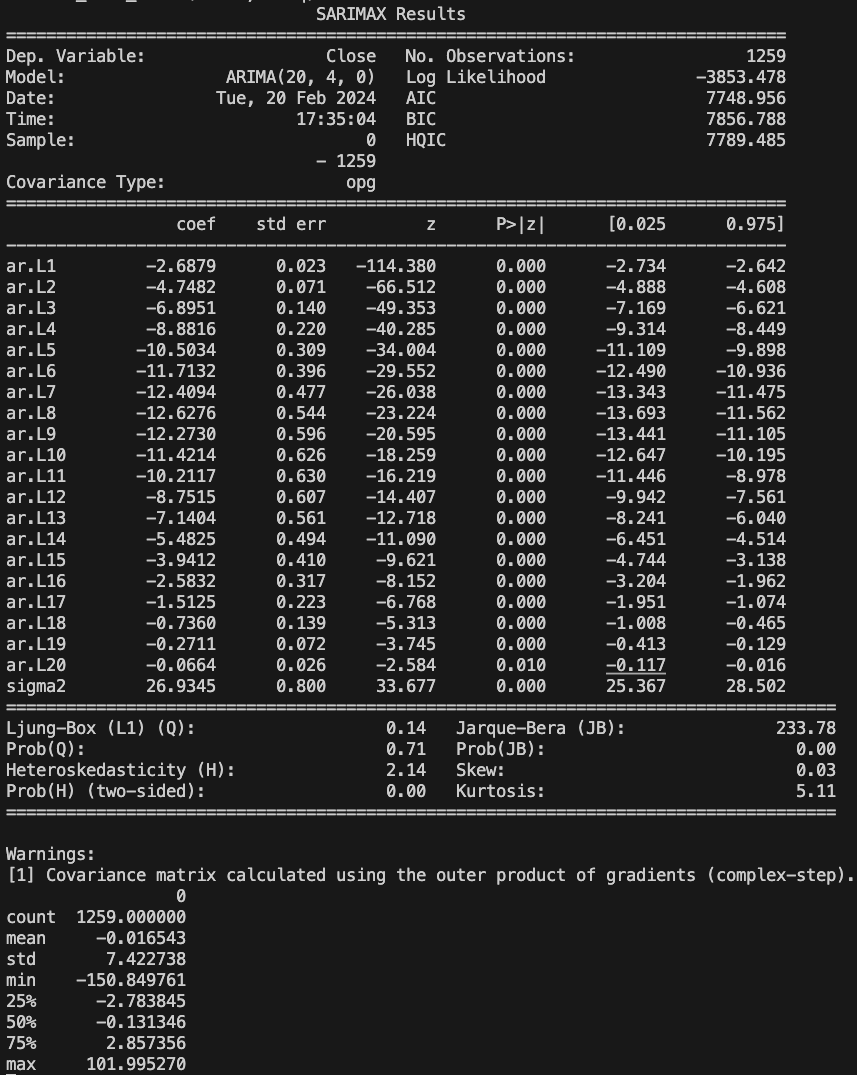
\includegraphics[width=0.8\textwidth]{ARIMA3.png}
                \caption{Risultati analisi preliminare della libreria 
                ARIMA}
            \end{figure}
            \begin{figure}[H]
                \centering
                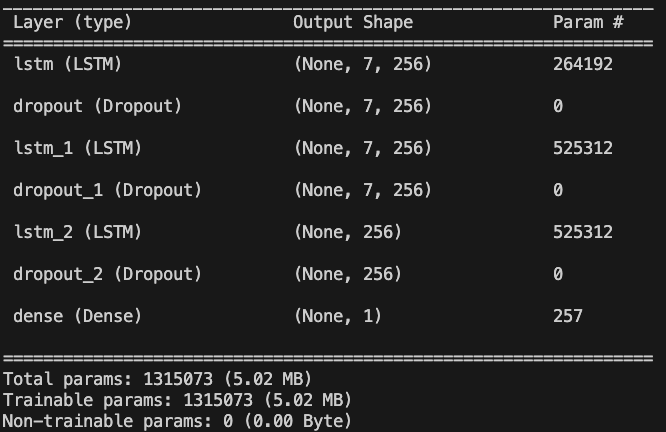
\includegraphics[width=0.8\textwidth]{LSTM3-1.png}
                \caption{Struttura Rete Neurale}
            \end{figure}
            \begin{figure}[H]
                \centering
                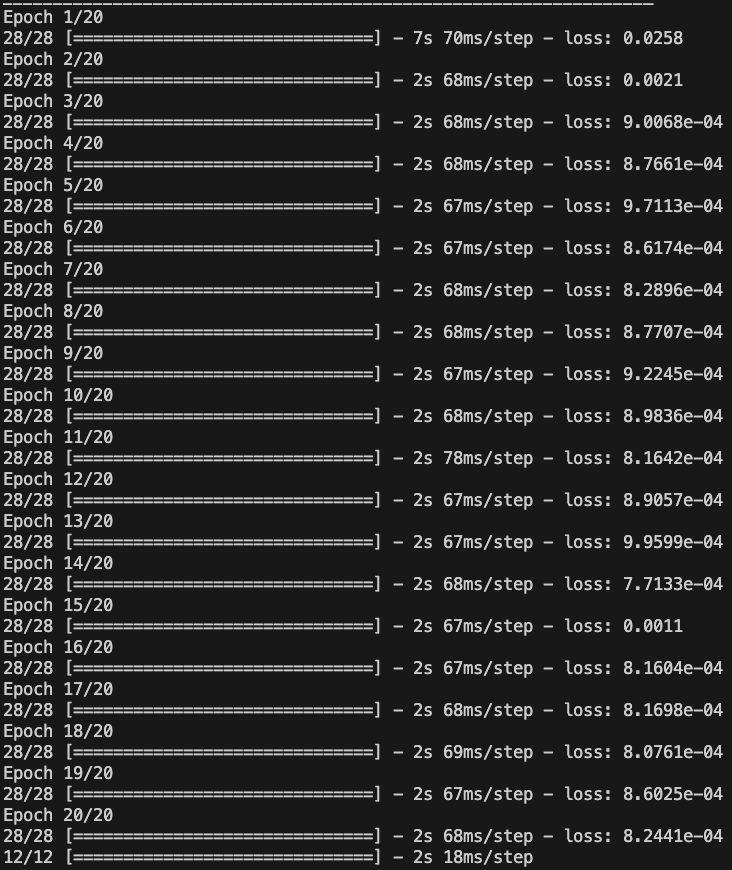
\includegraphics[width=0.6\textwidth]{LSTM3-2.png}
                \caption{Passi di addestramento}
            \end{figure}
            \begin{figure}[H]
                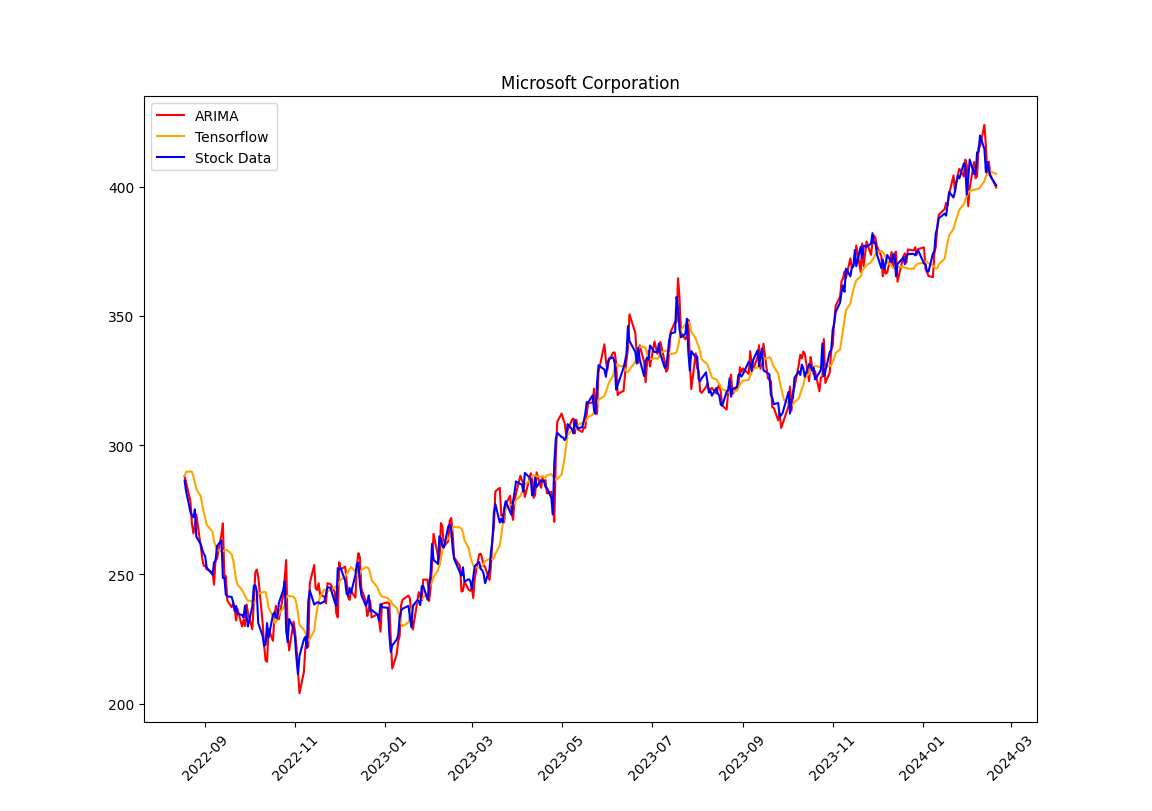
\includegraphics[width=\textwidth]{GRAFICO3.png}
                \caption{Confronto tra apprendimento ARIMA e LSTM}
            \end{figure}
            I risultati ottenuti, confrontati tramite scarto quadratico medio
            sono i seguenti:
            \begin{figure}[H]
                \centering
                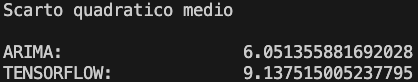
\includegraphics[width=0.5\textwidth]{SQM3.png}
                \caption{Confronti tra gli scarti quadratici medi}
            \end{figure}

    \section{Analisi risultati}Come possiamo notare, fin dai primi valori
    ottenuti tramite ARIMA, lo scarto quadratico medio è davvero basso, 
    ottenendo una curva di predizione quasi identica alla curva dei dati 
    originale. Incrementando i valori, per semplicità raddoppiati ad ogni
    addestramento, il valore dello scarto quadratico medio aumenta 
    anche se di poco.\\
    L'addestramento mediante Rete Neurale (Tensorflow LSTM), inizialemente
    ottiene prestazioni nettamente inferiori rispetto ad ARIMA. Questo possiamo
    tranquillamente notarlo con il divario che abbiamo tra i due scarti 
    quadratici medi. Tuttavia notiamo come all'aumentare della complessità 
    nella rete neurale, lo scarto quadratico medio diminuisce notevolemente.

    \section{Conclusioni}ARIMA applica una regressione specifica per le serie 
    temporali, di conseguenza possiamo notare come fin dai primi risultati 
    otteniamo previsioni ottime con scarti quadratici medi davvero bassi.\\
    LSTM invece utilizza comunque regressione ma per raggiungere la stessa 
    precisione (se non migliore di ARIMA), necessita di una complessità della 
    rete maggiore e una notevole quantità di potenza di calcolo (oltre che di 
    memoria) essendo una rete neurale applicabile sia a casi di regressione su 
    serie temporali, ma anche in riconoscimento della scrittura, delle parole e
    molti altri ambiti di ricerca.\\
    Nel caso di ARIMA, aumentando principalmente il valore di Autoregressione 
    (AR), otteniamo una complessità del polinomio maggiore aumentando di
    conseguenza lo scarto dai dati originali. Nella Rete Neurale abbiamo quindi
    un comportamento opposto dove, aumentando la complessità e la potenza di 
    calcolo richiesta, aumentiamo la precisione della nostra previsione 
    facendo diminiure lo scarto.\\
    Di fatti la Rete Neurale pur ricevendo un gran contributo da iperparametri
    come EPOCHS e SIZE, gran parte della precisione è affidata 
    all'iperparametro UNITS (che regola la dimensione di una singola cella 
    LSTM): notiamo difatti come aumentando la UNITS, a discapito della stessa
    SIZE per ogni confronto, vediamo come la dimensione degli input aumenta
    (da KB a MB) dato che, aumentando la complessità della cella, aumenta la
    complessità generale di come gli input vengono combinati ottenendo
    cammini computazionali più complessi e aumentando la precisione finale.
    L'iperparametro DROPOUT permette di scartare una serie di dati espressa in
    percentuale [0, 1] alleggerendo l'addestramento, esso è comunque 
    strettamente legato a UNITS difatti riducendo il suo valore verranno 
    scartati meno elementi. Ricollegandosi quindi a quanto detto 
    precedentemente, scartando meno dati, manteniamo cammini computazionali più
    complessi aumentando la precisione dell'addestramento (e di conseguenza
    il risultato finale).


\end{document}